\chapter{Introdução}

O projeto proposto visa o desenvolvimento de um sistema de telemedicina para a realização a distância. Por sua vez, o exame de ultrassom consiste em um método de exame não invasivo, indolor e barato (quando comparado a outros tipos de exame); ele produz imagens em tempo real de estruturas e órgãos internos. O aparelho de ultrassom tem como base o efeito doppler e ele é feito ao deslizar um pequeno aparelho transdutor sobre a pele do paciente, o qual emite ondas sonoras de alta frequência (2 a 20 MHz), que são captadas novamente no próprio aparelho sob a forma de eco \cite{ultrasomexame}.

Nesse contexto, o grupo visou desenvolver um braço para a movimentação automática do transdutor (sistema escravo) controlado a distância por uma estação de teleoperação (sistema principal). Dessa forma, considerando o Brasil como área de implementação do sistema, o braço controlado ficará em uma localidade brasileira onde não há grande disponibilidade de profissionais da saúde mas dispõe de internet cabeada de qualidade, como ocorre em grandes centros, permitindo assim, que uma população mais carente tenha acesso ao exame, sendo que o médico estará controlando o dispositivo a distância no próprio consultório.

Para atingir tal finalidade, a peça desenvolvida para a movimentação do transdutor deve reproduzir os movimentos que serão realizados pelas mãos do médico. Assim, a peça pensada é um braço robótico articulado, projetado e dimensionado para alcançar, com a movimentação do transdutor, uma área equivalente ao torso de uma pessoa.

Os transdutores que ele será capaz de segurar são o do aparelho de ultrassonografia Sonoscape A6, que suporta vários tipos de transdutores,o que será explicado mais à frente.

A aparência do braço é semelhante a descrita pela figura \ref{intr_fig1}. O funcionamento (movimentação) ocorre a partir de seis graus de liberdade, os quais determinam as condições de movimento da peça no espaço bidimensional ou tridimensional \cite{valdemircarrara2011}.

\begin{figure}[H]
	\centering	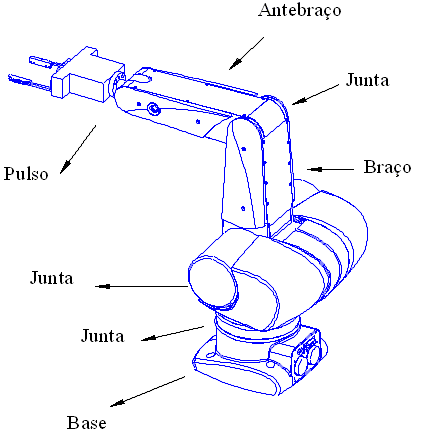
\includegraphics[keepaspectratio=true,scale=0.5]{figuras/braco_mecanico_1.png}
	\caption{Esquematização simples de um braço mecânico articulado \cite{valdemircarrara2011}}
	\label{intr_fig1}
\end{figure}

No sistema principal, a estação de teleoperação, é responsável pelo controle do movimento do braço, que será feito pelo médico. O médico terá em mãos um aparelho que simula um transdutor de ultrassonografia. A carcaça do aparelho terá o mesmo formato de um transdutor real, para a maior comodidade do operador. Dentro dessa carcaça será inserido um Arduino Nano juntamente com o módulo sensor inercial, escolhido para a captação dos movimentos do operador.

A carcaça é composta de dua partes iguais, que serão parafusadas uma contra a outra para comportar os componentes, que serão inseridos na cavidade retangular. A figura \ref{intr_fig2} a seguir mostra o modelo dessa carcaça.


       
\begin{figure}[H]
\centering
\begin{subfigure}{.5\textwidth}
  \centering
  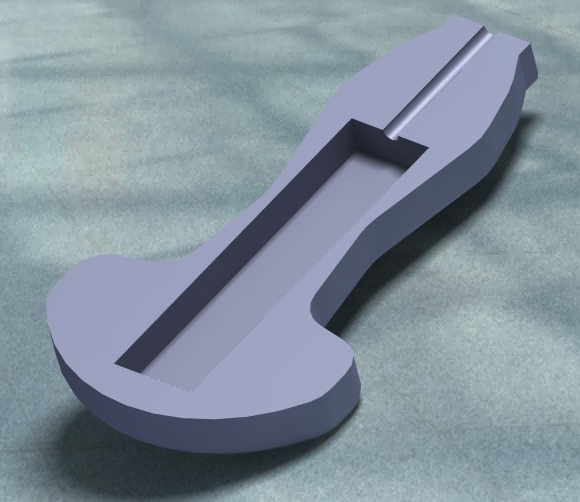
\includegraphics[width=.78\linewidth]{figuras/catia_controle_1.png}
  \caption{Carcaça do controle partida}
  \label{fig:sub1}
\end{subfigure}%
\begin{subfigure}{.5\textwidth}
  \centering
  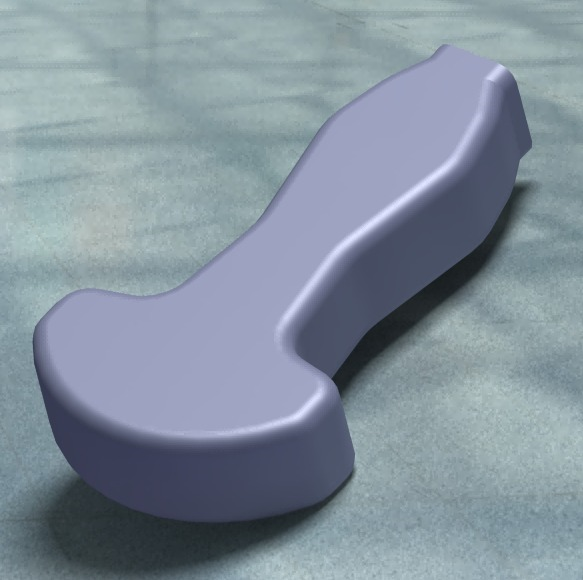
\includegraphics[width=.7\linewidth]{figuras/catia_controle_2.png}
  \caption{Carcaça do controle completa}
  \label{fig:sub2}
\end{subfigure}
\caption{Modelo CAD da carcaça}
\label{intr_fig2}
\end{figure}

O sistema escravo, além de incluir o braço mecânico movimentado por motores de passo e um sistema de ultrassom portátil comercial descrito anteriormente, é supervisionado por um profissional capacitado. Ele tem a função de transportar o braço mecânico para o local escolhido, monta-lo e ligar os equipamentos eletrônicos ao notebook, conectado este notebook a rede de internet cabeada local e preparar o paciente no local para realização do exame. Durante a realização do exame este profissional tem a função de supervisionar o exame e realizar controle de funções específicas, se necessário, no teclado do sistema de ultrassom que não seja possível remotamente realizado pelo médico.    

A comunicação entre o sistema principal e o sistema escravo será feita por meio de transmissão de comandos e imagens entre as unidades, utilizando a arquitetura de soquetes de internet. Será aberta uma linha de comunicação entre duas unidades utilizando a biblioteca socket do python, que oferece todas as ferramentas para configurar e utilizar a arquitetura de soquetes.

Os comandos de controle gerados pelo médico serão enviados para o servidor redirecionar a unidade de ultrassom através do canal de comunicação de soquete, que irá interpretar essa ordem e responderá de acordo. As imagens geradas pelo aparelho de ultrassom e a câmera ambiente também utilizarão desse canal para chegar  a unidade de controle da forma mais rápida. 

Dessa forma, a figura \ref{intr_fig3} a seguir exemplifica essa comunicação entre as unidades.

\begin{figure}[H]
	\centering	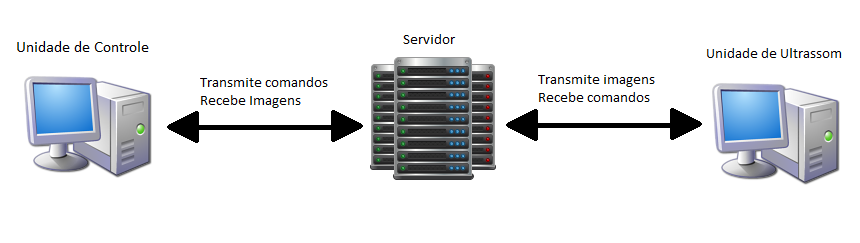
\includegraphics[keepaspectratio=true,scale=0.6]{figuras/1_0_comunicacao_socket.png}
	\caption{Comunicação via soquete}
	\label{intr_fig3}
\end{figure}

Já a alimentação energética será feita por meio de de tomadas de 110V ou de 220V de corrente alternada, tanto para a unidade principal, quanto para a unidade escrava. Entretanto como o arduino, que é o microcontrolador funciona com uma faixa de tensão de 6 a 20V com corrente contínua, há a necessidade de formas de proteção para o arduino, sendo elas um transformador de tensão e um circuito retificador de onda. Assim, o caminho que a energia deve percorrer até chegar ao microcontrolador é: tomada de 110V ou 220V$\longrightarrow$transformador$\longrightarrow$retificador de onda$\longrightarrow$arduino.

    Entretanto, para segurança do paciente, foi pensada fontes energéticas secundárias, sendo elas uma bateria tanto para o sistema escravo, quanto para o principal e uma placa solar para o sistema escravo. A razão dessas escolhas e seus funcionamentos serão explicadas posteriormente.
